
% Template for Elsevier CRC journal article
% version 1.1 dated 16 March 2010

% This file (c) 2010 Elsevier Ltd.  Modifications may be freely made,
% provided the edited file is saved under a different name

% This file contains modifications for Procedia Computer Science
% but may easily be adapted to other journals

% Changes since version 1.0
% - elsarticle class option changed from 1p to 3p (to better reflect CRC layout)

%-----------------------------------------------------------------------------------

%% This template uses the elsarticle.cls document class and the extension package ecrc.sty
%% For full documentation on usage of elsarticle.cls, consult the documentation "elsdoc.pdf"
%% Further resources available at http://www.elsevier.com/latex

%-----------------------------------------------------------------------------------

%%%%%%%%%%%%%%%%%%%%%%%%%%%%%%%%%%%%%%%%%%%%%%
%%%%%%%%%%%%%%%%%%%%%%%%%%%%%%%%%%%%%%%%%%%%%%
%%                                          %%
%% Important note on usage                  %%
%% -----------------------                  %%
%% This file must be compiled with PDFLaTeX %%
%% Using standard LaTeX will not work!      %%
%%                                          %%
%%%%%%%%%%%%%%%%%%%%%%%%%%%%%%%%%%%%%%%%%%%%%%
%%%%%%%%%%%%%%%%%%%%%%%%%%%%%%%%%%%%%%%%%%%%%%

%% The '3p' and 'times' class options of elsarticle are used for Elsevier CRC
\documentclass[3p,times,authoryear]{elsarticle}

%% The `ecrc' package must be called to make the CRC functionality available
\usepackage{ecrc}
\usepackage{amsmath}

%% The ecrc package defines commands needed for running heads and logos.
%% For running heads, you can set the journal name, the volume, the starting page and the authors

%% set the volume if you know. Otherwise `00'
\volume{00}

%% set the starting page if not 1
\firstpage{1}

%% Give the name of the journal
\journalname{Chemical Engineering Science}

%% Give the author list to appear in the running head
%% Example \runauth{C.V. Radhakrishnan et al.}
\runauth{}

%% The choice of journal logo is determined by the \jid and \jnltitlelogo commands.
%% A user-supplied logo with the name <\jid>logo.pdf will be inserted if present.
%% e.g. if \jid{yspmi} the system will look for a file yspmilogo.pdf
%% Otherwise the content of \jnltitlelogo will be set between horizontal lines as a default logo

%% Give the abbreviation of the Journal.
\jid{procs}

%% Give a short journal name for the dummy logo (if needed)
\jnltitlelogo{Procedia Computer Science}

%% Hereafter the template follows `elsarticle'.
%% For more details see the existing template files elsarticle-template-harv.tex and elsarticle-template-num.tex.

%% Elsevier CRC generally uses a numbered reference style
%% For this, the conventions of elsarticle-template-num.tex should be followed (included below)
%% If using BibTeX, use the style file elsarticle-num.bst

%% End of ecrc-specific commands
%%%%%%%%%%%%%%%%%%%%%%%%%%%%%%%%%%%%%%%%%%%%%%%%%%%%%%%%%%%%%%%%%%%%%%%%%%

%% The amssymb package provides various useful mathematical symbols
\usepackage{amssymb}
\usepackage{natbib}
\bibliographystyle{apalike}
\setcitestyle{authoryear,open={(},close={)}}
%% The amsthm package provides extended theorem environments
%% \usepackage{amsthm}

%% The lineno packages adds line numbers. Start line numbering with
%% \begin{linenumbers}, end it with \end{linenumbers}. Or switch it on
%% for the whole article with \linenumbers after \end{frontmatter}.
%% \usepackage{lineno}

%% natbib.sty is loaded by default. However, natbib options can be
%% provided with \biboptions{...} command. Following options are
%% valid:

%%   round  -  round parentheses are used (default)
%%   square -  square brackets are used   [option]
%%   curly  -  curly braces are used      {option}
%%   angle  -  angle brackets are used    <option>
%%   semicolon  -  multiple citations separated by semi-colon
%%   colon  - same as semicolon, an earlier confusion
%%   comma  -  separated by comma
%%   numbers-  selects numerical citations
%%   super  -  numerical citations as superscripts
%%   sort   -  sorts multiple citations according to order in ref. list
%%   sort&compress   -  like sort, but also compresses numerical citations
%%   compress - compresses without sorting
%%
%% \biboptions{comma,round}

%\biboptions{sort&compress,comma}

% if you have landscape tables
\usepackage[figuresright]{rotating}
\usepackage{cleveref}
\usepackage{float}
% put your own definitions here:
%   \newcommand{\cZ}{\cal{Z}}
%   \newtheorem{def}{Definition}[section]
%   ...

% add words to TeX's hyphenation exception list
%\hyphenation{author another created financial paper re-commend-ed Post-Script}

% declarations for front matter
%\bibliographystyle{elsarticle-num}
\begin{document}

\begin{frontmatter}

%% Title, authors and addresses

%% use the tnoteref command within \title for footnotes;
%% use the tnotetext command for the associated footnote;
%% use the fnref command within \author or \address for footnotes;
%% use the fntext command for the associated footnote;
%% use the corref command within \author for corresponding author footnotes;
%% use the cortext command for the associated footnote;
%% use the ead command for the email address,
%% and the form \ead[url] for the home page:
%%
%% \title{Title\tnoteref{label1}}
%% \tnotetext[label1]{}
%% \author{Name\corref{cor1}\fnref{label2}}
%% \ead{email address}
%% \ead[url]{home page}
%% \fntext[label2]{}
%% \cortext[cor1]{}
%% \address{Address\fnref{label3}}
%% \fntext[label3]{}

\dochead{}
%% Use \dochead if there is an article header, e.g. \dochead{Short communication}

\title{Deterministic and Stochastic Optimal Control for Batch Cooling Crystallization}

%% use optional labels to link authors explicitly to addresses:
%% \author[label1,label2]{<author name>}
%% \address[label1]{<address>}
%% \address[label2]{<address>}

\author{Tushar Gupta}

\address{}

\begin{abstract}
This paper presents a stochastic model predictive control(MPC) approach for nonlinear systems which are subject to time-invariant probabilistic uncertainties in model parameters. The field under study here is batch crystalllization which is affected heavily by the uncertainities in model parameters which leads to sub-par performace in process operation. Uncertanity quantification helps to mitigate this problem by by incorporating the errors, in the optimization algorithms while performing predictive control. Each of the optimization algorithms entail a cost function which maximises the amount or the expected value of the desired product. First, this work presents a determistic study to highlight the kinetics of the batch process and then draws comparison with the stochastic process to indicate an increase in performance in the later. The dynamic uncertainities in the process are modeled using Ito's lemma, stochastic calculus and stochastic maximum princile. In the end, a novel approach named Polynomial Chaos Expansions is implemented for the control strategy, which has been applied successfully to other domains for nonlinear MPC but was not explored in detail in the field of batch cooled crystalllization. It successfuly includes probability distributions for the parameters into the model to provide a more robust optimization srategy. 
 %The key challenge in addressing robustness to model
%error is to propagate the uncertainty in model parameters onto the
%%control or optimization objective.

\end{abstract}

\begin{keyword}
Stochastic Optimal Control \sep Polynomial Chaos Expansions \sep Robust Optimization \sep Batch Crystallization \sep Predictive Control
\sep Optimum Temperature Profile
%% keywords here, in the form: keyword \sep keyword

%% MSC codes here, in the form: \MSC code \sep code
%% or \MSC[2008] code \sep code (2000 is the default)

\end{keyword}

\end{frontmatter}

%%
%% Start line numbering here if you want
%%
% \linenumbers

%% main text
\section{Introduction}
\label{intro}
Numerous industries today, such as pharmaceutical, chemical, photographic etc. employ the batch crystallization process for the preparation of crystalline products with high degree of purity. A common goal of each crystallization process is to obtain a narrower Particle size distribution (PSD) of the desired product. The PSD has a strong influence on the downstream processing and, hence, reproducible PSD in each operation is of prime importance. Thus, finding an effective control strategy to obtain the resulting crystals with a desired Crystal Size Distribution becomes significant in order for improving the performance of both the batch crystallization process and the subsequent processes which depend on it. \par
Crystallization is the (natural or artificial) process where the atoms or molecules are highly organized into a solid structure known as a crystal. Some of the ways which crystals form are through precipitating 
from a solution, melt or more rarely deposited directly from a gas. In order for crystallization to take place a solution must be "\textit{supersaturated}". \textbf{Supersaturation}$(\Delta{C})$  is a condition in which the solute concentration in the solution is
higher than the solubility. It acts as the driving force for the crystallization process and affects the final quantity of product formed. It is mathematically expressed  as : 
\begin{equation}
\Delta{C} = C - C_{s}
\end{equation}
where $C_{s}$ is the concentration of the solute in the saturated solution.
In the following work, the method in focus is cooling crystallization in which superstauration magnitude is determined by the cooling rate. Thus, determination of an optimal cooling rate or a temperature trajectory becomes the objective of the currrent study. \par 
This work formulates and analyses various control strategies for a cooling crystallization process represented through the population balance equation. \textbf{Deterministic Optimal Control} aims at finding the an optimum temperature profile to maximise an objective function selected to achieve a desired volume of the product.
Herein, the experimental kinetic parameters are employed to simulate a batch crystalllization process. \textbf{Stochastic Optimal Control} undertakes the task of quantifying the uncertainites which creep in due to experimentation. It aims to achive a maximum expected value for the desired product, simultaneously incorporating randomness in the process parameters into the model. Namely, two methods \textbf{Ito Process} and a novel approach \textbf{Polynomial Chaos Expansions} are employed for this purpose. \par

Most of the reported works in the this field deal with the determination of optimal temperature or supersaturation trajectory for the batch crystallizer. The concept of programmed cooling in batch crystallizers was first discussed by \cite{mullin}.
Later, \cite{agjones} presented a mathematical theory based on moment transformations of population balance equations. He used the continuous maximum principle to predict optimal cooling curves.
\cite{rawlings} discussed issues in crystal size measurement using laser light scattering experiments and optimal control problem formulation. \cite{miller_rawlings}  discussed the uncertain bounds on model parameter estimates for a batch crystallization system. 
Most importantly optimal temperature prediction for batch crystallization has also been done by \cite{hu}, \cite{shi}, \cite{paeng} and \cite{corriou}, the data and knowledge from which have been used in further work in this project.\par
Stochastic modeling of particulate processes and parameter estimation using the experimentally measured particle sizes has attracted many researchers. \cite{grosso} presented a stochastic approach for modeling PSD and comparative assessments of different models. \cite{ma} presented a worse-case performance analysis of optimal control trajectories by considering features such as the computational effort, parametric uncertainty and control implementation inaccuracies. Monte Carlo simulations have also been used to propogate uncertainities but often present the problem of high computational demand, for which this work proposes Polynomial Chaos Expansions(PCEs) as an alternative. The computational advantages of PCEs for robust control and optimization has been shown by \cite{nagy}, \cite{kim} and \cite{kumar}. \par
The focus of the current research activity is to incorporate parametric uncertainties in the mathematical formulations of batch crystallization process for building a robust model. In the deterministic approach, kinetic parameters from the experimental data have been used to model the system. Next, stochastic Ito processes are used to assimilate the errors in the experimental data. Finally, PCE are demostrated as an effective method for non-linear optimization in batch reactors. A case study of an unseeded crystallization process is also included to authenticate the methodology.
%It is based on orthogonal basis functions thus requiring smaller function evaluations for the calculation of numerical integrations needed for obtaining statistical moments.

\section{Materials and methods} \label{model}

%\subsection{Seeded batch Crystallization} 

This section introduces the underlying concepts needed to build a computational model of a crystallization process which involves regulating the population of particles, also termed as a particulate process. 
The population is described by the density of a suitable extensive variable, usually the \textbf{number of particles}, but sometimes by other variables such as the mass or volume of particles. The usual transport equations expressing conservation laws for material systems apply to the behavior of single particles. Particulate processes are characterized by properties such as particle shape, size, surface area, mass, and product purity. \par
A population balance formulation describes the process of crystal size distribution with time most effectively. Thus, modeling of a batch crystallizer involves the use of population balances to model the crystal size prediction and the mass balance on the system can be modeled as a simple differential equation having concentration as the state variable.
The population balance can be expressed as eq :

\begin{equation} \label{populationbalance}
\frac{\partial{n(r,t)}}{\partial{t}} + \frac{\partial{G(r,t)n(r,t)}}{\partial{r}} = B  
\end{equation}
where \textbf{n} is the number density distribution, \textbf{t} is the time, \textbf{r} represents the characteristic dimension for size measurements, \textbf{G} is the crystal growth rate, and \textbf{B} is the nucleation rate. Both growth and nucleation processes describe crystallization kinetics, and their expression may vary, depending on the system under consideration.

In this work, the system under consideration is potassium sulfate, which has been studied earlier for its kinetics by \cite{hu}, \cite{shi} and \cite{paeng}. The equations expressing the kinetics and values for the kinetic parameters have been derived form these literary works. 

Nucleation kinetics are defined by :
\begin{equation}
B(t) = k_{b}\exp{\left(-E_{b}/RT \right)}\left(\frac{C - C_{s}(T)}{C_{s}(T)}\right)^{b}\mu_{3}
\end{equation}  


Growth Kinetics are given by:
\begin{equation}
G(t) = k_{g}\exp{\left(-E_{g}/RT \right)}\left(\frac{C - C_{s}(T)}{C_{s}(T)}\right)^{g}
\end{equation}
where k$_{b}$ and k$_{g}$ are constants of the system, E$_{b}$ and E$_{g}$ are activation energies, and b and g are exponents of nucleation and growth, respectively. The values for these parameters for the given system have been mentioned in Table \ref{Table1}. The following equations are used to evaluate the saturation($C_{s}$) and metastable($C_{m}$) concentrations corresponding to the solution temperature T (expressed in units of $^\circ$C) (\cite{shi}). \\
\begin{align}
C_{s}(T) &= 6.29\times10^{-2} + 2.46\times10^{-3}T - 7.14\times10^{-6}T^{2} \label{sat}\\
C_{m}(T) &= 7.76\times10^{-2} + 2.46\times10^{-3}T - 8.1\times10^{-6}T^{2} \label{meta}
\end{align}

 
The mass balance, in terms of concentration of the solute in the solution, is expressed as :
\begin{equation}
\frac{dC}{dt} = -3\rho{}k_{v}G(t)\mu_{2}(t)
\end{equation}
where $\rho{}$ is the density of the crystals, $k_{v}$ the volumetric shape factor, and $\mu_{2}$ is the second moment of particle size distribution (PSD).
Since $n(r,t)$ represents the population density of the crystals, the i-th moment of the particle size distribution(PSD) is given by :
\begin{equation} \label{moments}
\mu_{i} = \int_{0}^{\infty} r^{i}n(r,t) dr
\end{equation}
The above equations along with the Population Balance Equation(PBE) (\ref{populationbalance}) represent a complete model of a seeded batch crystallizer. 
Population balance equations are multidimensional, which poses a problem with their implementation in complex control functions, hence use of a model order reduction becomes imperative.\par
For simplification, we reduce the population balance equations into \textbf{Moment balance equations} which has been estabilished as an efficient method by \cite{yenkie}. This is done by multiplying the equation (\ref{populationbalance})  with $r^{i}$ on both sides to generate the expression given by equation (\ref{moments}). Converting the model into Ordinary differential equations proves to be advantageous, since it is difficult and time-consuming to formulate an optimization problem involving PBEs. Thus, the moment method leads to a reduced-order model given by \Crefrange{g1}{n1}

Separate moment equations are used for the seed and nuclei classes of crystals, and they are defined as : \\
\begin{align}
\mu^{n}_{i} &= \int_{0}^{r_{g}} r^{i}n(r,t) dr \\
\mu^{s}_{i} &= \int_{r_{g}}^{\infty} r^{i}n(r,t) dr
\end{align} \\
\textbf{n} in the superscript represents the nucleated crystal whereas \textbf{s} stands for the seeded crystal, $\boldsymbol{r_{g}}$ gives the critical radius separating the two. The resultatnt moment equations for nucleated and seeded crystals are as follows (\cite{yenkie}) :

\begin{enumerate}

\item Nucleated crystals
\begin{align}
\frac{d\mu_{0}^{n}}{dt} &= B(t) \label{g1} \\
\frac{d\mu_{i}^{n}}{dt} &= iG(t)u_{i-1}^{n}(t) \quad  i = 1,2,3
\end{align}

\item Seeded crystals
\begin{align}
\mu_{0}^{s} &= constant  \label{seed} \\ 
\frac{d\mu_{i}^{s}}{dt} &= iG(t)u_{i-1}^{n}(t) \quad  i = 1,2,3  \label{n1} 
\end{align}
\end{enumerate}
The total moment is obtained as the summation $\mu_{i}^{t} = \mu_{i}^{n} + \mu_{i}^{s}$. Here, $\mu_{0}^{s}$ represents the amount of seeded crystals and hence remains constant. Also, fourth-order moments and higher do not affect third-order moments and lower, implying that only the first four moments and concentration can adequately represent the crystallization dynamics (\cite{shi}). 
\par
The crystallization model defined above has been used to compare the performance of different types of optimization techniques, both in the deterministic and stochastic domain, which is explained in detail in the susequent sections.
\begin{center}
\begin{table}[!h]
\centering
\caption{Experimental values of Kinetic Parameters}
\begin{tabular}{|c|c|}
\hline
Parameters & Experimental Values \\
\hline
\multicolumn{2}{|c|}{Growth Kinetics} \\
\hline
$k_{g}$ & $1.44\times10^{8} \mu m s^{-1}$ \\
$E_{g}/R$ & $4859K$ \\
$g$ & $1.5$ \\
\hline
\multicolumn{2}{|c|}{Nucleation Kinetics} \\
\hline
$k_{b}$ & $285 (s \mu m^{3})^{-1}$ \\ 
$E_{b}/R$ & $7517K$ \\
$b$ & $1.45$ \\
\hline
\end{tabular}
\label{Table1}
\end{table}
\end{center}
\section{Deterministic Optimal Control}\label{secdet}

\subsection{\textit{Case Study : Seeded batch crystallization}}
Optimal control involves the evaluation of time-dependent operating profiles, in terms of the control variable to optimize the process performance. In the crystallization domain, temperature becomes the control variable while the product yield is used to evaluate the performance of the model. The Optimization problem here is solved by using the method of Maximum Principle as discussed extensively by \cite{diwekar}. This method stands out in compared to other techniques such as dynamic programming as it involves the use of first order ODEs while the later utilises partial differential equations. Another advantage of maximum principle is its ability to adapt to stochastic calculus which is explained in the next section. \par 
In a seeded crystallization process it is essential to keep the nucleation phenomena to minimum as in the early stages of growth, nucleated crystals might compete with the seeded ones for growth. This ensures uniformity in the shape and size of the final product. It is achieved by incorporating the volume of nucleated in the \textbf{objective fuction}. Third moment($\mu_{3}$) represents volume in a crystallization model as evident from Equation(\ref{moments}) and is used as follows :
\begin{equation}
\max_{T(t)}\lbrace{\mu_{3}^{s}(t_{f}) - \mu_{3}^{n}(t_{f})\rbrace } 
\end{equation}
The active constraints for the process are given by : 
\begin{equation}
C_{s}\leqslant C \leqslant C_{m}
\end{equation}
$C_{m}$ is the metastable concentration described by Equation(\ref{meta}). The state variables $y_{i}$ for the process are now representes as : 
\begin{equation} \label{states}
y_{i} = \left[\quad C \quad \mu_{0}^{s} \quad \mu_{1}^{s}\quad \mu_{2}^{s}\quad \mu_{3}^{s}\quad \mu_{0}^{n}\quad \mu_{1}^{n}\quad \mu_{2}^{n}\quad \mu_{3}^{n}\quad\right]  
\end{equation}
Using the above notations the state equations can be realized as (\cite{yenkie}) :
\begin{align} 
\frac{dy_{1}}{dt} &= -3\rho k_{v}G(t)(y_{4}+y_{8}) \label{eq1}\\
\frac{dy_{2}}{dt} &= 0 \label{eq2}\\
\frac{dy_{3}}{dt} &= G(t)y_{2} \label{eq3} \\
\frac{dy_{4}}{dt} &= 2G(t)y_{3} \label{eq4}\\
\frac{dy_{5}}{dt} &= 3G(t)y_{4} \label{eq5}\\
\frac{dy_{6}}{dt} &= B(t)  \label{eq6}\\
\frac{dy_{7}}{dt} &= G(t)y_{6}  \label{eq7}\\
\frac{dy_{8}}{dt} &= 2G(t)y_{7} \label{eq8} \\
\frac{dy_{9}}{dt} &= 3G(t)y_{8} \label{eq9} \\
\end{align} 


Thus, the complete model involving the moment equations consists of nine state equations.
\subsection{\textit{Solution technique}} \label{soltech} 

The algorithm of Steepest Ascent utilizes the Maximum Principle using the Hamiltonian to move towards the optimum value of temperature and maximise the objective function. To formulate the equations an adjoint varible ($z_{i}$) is defined corresponding to each state variable ($y_{i}$) The adjoint variable staisfy the relations given by eq \ref{adjoints}. Using the state and the adjoint equations, a two-point boundary-value-problem is constructed. Here, the intial values for the states and the final conditions for the adjoint variables are known beforehand.
The Hamiltonian can now be defined by eq \ref{hamilt}.
\begin{equation} 
H = \sum_{i = 1}^{9} z_{i}f(y_{i},t,T) \label{hamilt}
\end{equation}
The complete model with the objective function is given by \Crefrange{obj}{adjoints}:
\begin{equation} \label{obj}
max_{T(t)} \lbrace{ y_{5}(t_{f}) - y_{9}(t_{f})}\rbrace 
\end{equation}
\begin{equation}
\frac{dy_{i}}{dt} = f(y_{i},t,T) 
\end{equation}
\begin{equation} \label{adjoints}
\frac{dz_{i}}{dt} = \sum_{j=1}^{9} z_{j}\frac{\partial f(y_{i},t,T)}{\partial y_{i}} = f(y_{i},z_{i},t,T) 
\end{equation}
with the initial and final conditions:
\begin{align*}
&t_{0} = 0 \quad and \quad t_{f} = 1800s \quad(batch \quad time) \\
&y_{i}(t_{0}) = \left[ 0.1743 \quad 66.66 \quad 1.83\times10^{4}\quad 5.05\times10^{6} \quad 1.93\times10^{9} \quad 0.867 \quad 0 \quad 0 \quad 0 \right] \\
&z_{i}(t_{f}) = \left[  0 \quad 0 \quad 0 \quad 0 \quad 1 \quad 0 \quad 0 \quad 0 \quad -1 \right] 
\end{align*}
The steps followed to solve the optimal control problem have been discussed in detail below.
\begin{enumerate}
\item An initial temperature $T(t) = 323 K$ is assumed for the entire time horizon.
\item The differential equations for state variables($y_{i}$) are integrated in the forward direction using the given initial conditions.
\item The values of the adjoint variables($z_{i}$) are computed by backward integration of the adjoint equations given by eqs. \ref{adjoints}.
\item For evaluation of the Hamiltonian derivative, an analytical method proposed by \cite{benavides}, is used in which an additional variable corresponding to each of the state and adjoint variable is introduced. The variable $\theta_{i}$ corresponds to each of the state variable $y_{i}$ and the variable $\phi_{i}$ corresponds to each of the adjoint variable $z_{i}$, which is given by eq(\ref{thetafi}).
\begin{equation}
\theta_{i} = \frac{dy_{i}}{dT} \quad and \quad \phi_{i} = \frac{dz_{i}}{dT} \label{thetafi} 
\end{equation}
\item The variables $\theta_{i}$ and $\phi_{i}$ along with $y_{i}$ and $z_{i}$ give the derivative of Hamiltonian by \ref{hamiltd}. The differential equaltions used for computing $\theta_{i}$ and $\phi_{i}$ are obtained by the following method :  
\begin{align}
\frac{d\left( \frac{dy_{i}}{dt}  \right)}{dT} &= \frac{d\left( \frac{dy_{i}}{dT}  \right)}{dt} = \frac{d\theta_{i}}{dt} \label{theta}\\
\frac{d\left( \frac{dz_{i}}{dt}  \right)}{dT} &= \frac{d\left( \frac{dz_{i}}{dT}  \right)}{dt} = \frac{d\phi_{i}}{dt} \label{phi}
\end{align}
The intial conditions used for forward integration of $\frac{d\theta_{i}}{dt}$ are $\theta_{i}(t_{0}) = \left[  0 \quad 0 \quad 0 \quad 0 \quad 0 \quad 0 \quad 0 \quad 0 \quad 0 \right]$ and the final conditions used for the backward integration of $\frac{d\phi_{i}}{dt}$ are $\phi_{i}(t_{f}) = \left[  0 \quad 0 \quad 0 \quad 0 \quad 0 \quad 0 \quad 0 \quad 0 \quad 0 \right]$  
\item The Hamiltonian derivative is now calculated at each time step by \ref{hamiltd}. 
\begin{align}
\frac{dH}{dT} &= \sum_{i=1}^{9} \left( \frac{dH}{dy_{i}}\right)\left(	\frac{dy_{i}}{dT} \right) + \sum_{i=1}^{9} \left(\frac{dH}{dz_{i}}\right)\left(\frac{dz_{i}}{dT} \right) \\
\frac{dH}{dT} &= \sum_{i=1}^{9} \left( \frac{dH}{dy_{i}}\right) \theta_{i}  + \sum_{i=1}^{9} \left(\frac{dH}{dz_{i}}\right) \phi_{i}  \label{hamiltd} 
\end{align}
\item The computed value of the derivative is checked against the convergence criterion $(\frac{dH}{dT}<$ tolerance). If it is not satisfied, the temperature $T(t)$ is updated using eq(\ref{temp}). This ensures that the optimal control variable $T(t)$ is obtained using the extremum of hamiltonian. 
\begin{equation} 
T^{new}(t) = T^{old}(t) + M\left(\frac{dH}{dT} \right) \label{temp}
\end{equation}
\item The concentration is evaluated  at that time step and compared with first with the saturation concentration ($C_{s}$) and then the metastable concentration($C_{m}$) to validate the active constraints. If it found to be lesser than saturation value or greater than the metastable value, eqs (\ref{sat}) and (\ref{meta}) are used to compute the new temperature respectively. 
\item Iterations of above steps are repeated until the convergence criteria is achieved.
\end{enumerate}

\subsection{\textit{Results}}
%%% >>>>>>>>>>>>>>> Change to Matlab
The integration of differential equations was performed in python using the odeint routine from the scipy open source package.
The resultant optimal temperature profile is shown in Figure (\ref{Dtemp}). The system attains a constant value of $300 K$ at $\sim1700 s$. The decreasing temperature profile is indicative of the cooling crystallization. Also, the objective function can be observed to reach a maximum value in the Figure(\ref{Dobj}). The concentration profile of solute in the system is given by the Figure(\ref{Dconc}). 
%The change of the Hamiltonian Derivative($\frac{dH}{dT}$) after each iteration can be seen from Figures (\ref{it1})-(\ref{it2}). After the final iteration, values of the derivative converge within tolerance limits which signifies reaching an optimal point.

\begin{figure}[H] 
\begin{center}
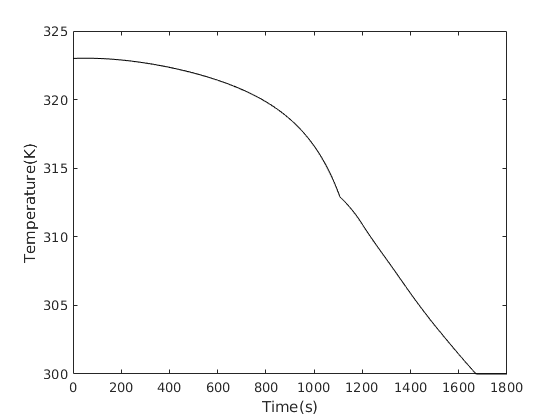
\includegraphics[width=4in]{images/Dtemp.eps}
\end{center}
\caption{The cooling profile for the controlled variable T(t) obtained at the final iteration} \label{Dtemp}
\end{figure}

\begin{figure}[h!] 
\begin{center} 
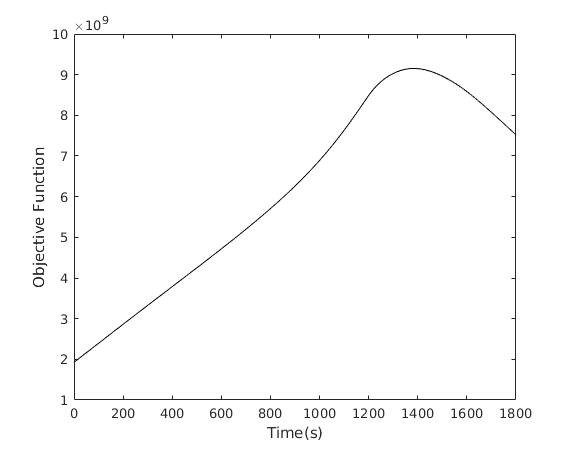
\includegraphics[width=4in]{images/Dobj.eps}
\end{center}
\caption{Objective Function ($\mu_{3}^{s}(t) - \mu_{3}^{n}(t)$)} \label{Dobj}
\end{figure}
%\begin{figure}[h!] \label{it1}
%  \centering 
%  \begin{minipage}[b]{0.4\textwidth}
%    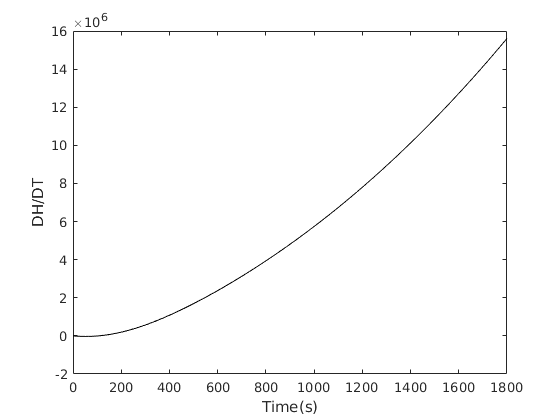
\includegraphics[width=\textwidth]{images/h1.eps}
%    \caption{Iteration 1}
%  \end{minipage}
%  \hfill
%  \begin{minipage}[b]{0.4\textwidth}
%    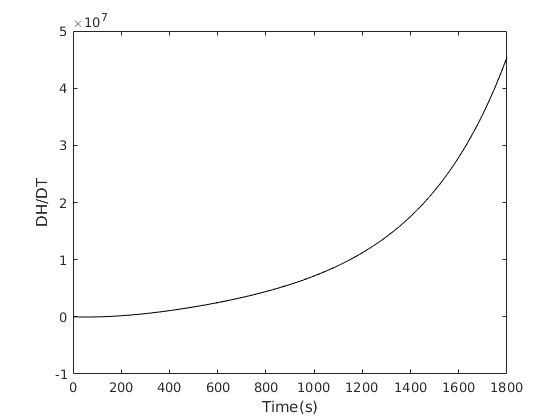
\includegraphics[width=\textwidth]{images/h2.eps}
%    \caption{Iteration 2}
%  \end{minipage}
%\end{figure}
%\begin{figure}[h!]
%  \centering
%  \begin{minipage}[b]{0.4\textwidth}
%    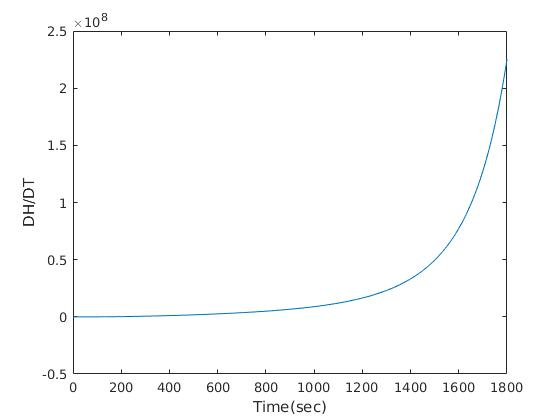
\includegraphics[width=\textwidth]{images/h3.eps}
%    \caption{Iteration 3}
%  \end{minipage}
%  \hfill
%  \begin{minipage}[b]{0.4\textwidth}
%    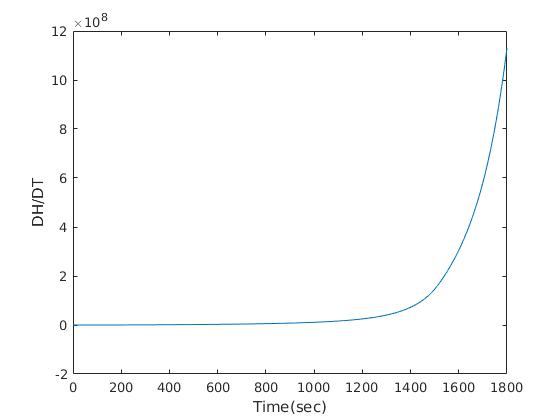
\includegraphics[width=\textwidth]{images/h4.eps}
%    \caption{Iteration 4}
%  \end{minipage}
%\end{figure}
%\begin{figure}[h!]
%  \centering
%  \begin{minipage}[b]{0.4\textwidth}
%    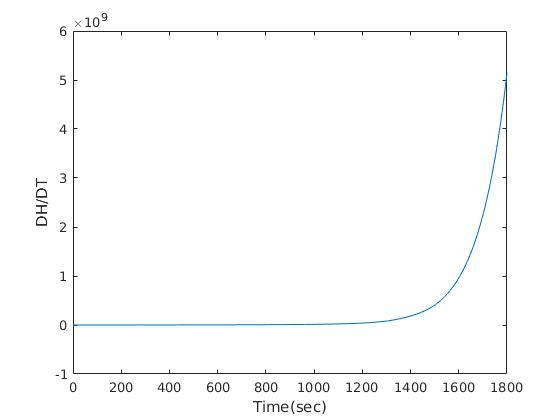
\includegraphics[width=\textwidth]{images/h5.eps}
%    \caption{Iteration 5}
%  \end{minipage}
%  \hfill
%  \begin{minipage}[b]{0.4\textwidth}\label{it2}
%    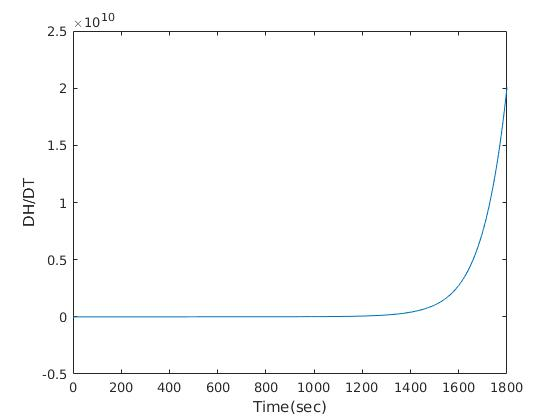
\includegraphics[width=\textwidth]{images/h6.eps}
%    \caption{Iteration 6}
%  \end{minipage}
%\end{figure}

\begin{figure}[h!] 

\begin{center} 
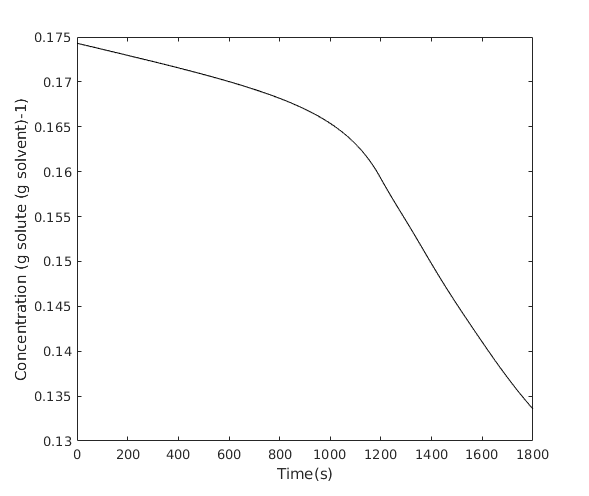
\includegraphics[width=4in]{images/Dconc.png}
\end{center}
\caption{The Concentration profile as obtained.} \label{Dconc}
\end{figure}

\section{Optimal Control using Uncertainity Quantification}


The kinetic parameters used in the Section(\ref{secdet}) are empirical constants which are obtained through experimentation and hence, are a source of errors into the model. The exact values of the parameters are unknown and thus are termed as uncertainties which go on to produce sub-optimal results when used in real-world applications. In the next section, we convert the deterministic problem into a stochastic one, wherein the kinetic constants are treated as random variables to include variation in there values into the final output produced by the model. Thus, two methods are analysed to address the given problem. 

\subsection{Stochastic Optimal Control using Ito Processes}

%%%%%
% Give proper  references here 
%%%%%
Several previous works have shown that the dynamic uncertainties present in batch reactors (\cite{benavides}) and batch distillations (\cite{diwekar}), can be represented using stochastic processes known as Ito processes. We characterize the time-dependent uncertainties in the state variables using Ito processes known as Brownian motion with drift (\cite{diwekar,wong}). The advantage lies in the ability to integrate the equations through the principles of stochastic calculus and the use of stochastic maximum principle to solve for the optimal temperature profile. 
A simple Ito process can be written as eq (\ref{gen})
\begin{equation} \label{gen}
dy = a(y,t)dt + b(y,t)dz
\end{equation}
where $dz$ is the increment of the Wiener process equal to $\varepsilon_{t}(\Delta t)^{1/2}$, and a(y,t) and b(y,t) are known functions. The random value $\varepsilon_{t}$ has a unit normal distribution with zero mean and a standard deviation of 1. To estimate the values of the functions a and b, a generalized method presented by \cite{diwekar} has been used.\par
In this work, equation(\ref{gen}) is used to modify the deterministic state (\Crefrange{eq1}{eq9}) to incorporate the uncertainties into the moment equations as follows :
\begin{align}
dy_{1} &= \left(-3\rho k_{v}G(t)(y_{4}+y{8})\right)\Delta t + g_{1}\varepsilon_{1}\sqrt{\Delta t} \label{steq1}\\
dy_{2} &= 0 \\
dy_{3} &= (G(t)y_{2})\Delta t +g_{3}\varepsilon_{3}\sqrt{\Delta t} \\
dy_{4} &= (2G(t)y_{3})\Delta t + g_{4}\varepsilon_{4}\sqrt{\Delta t} \\
dy_{5} &= (3G(t)y_{4})\Delta t + g_{5}\varepsilon_{5}\sqrt{\Delta t} \\
dy_{6} &= (B(t))\Delta t + g_{6}\varepsilon_{6}\sqrt{\Delta t} \\
dy_{7} &= (G(t)y_{6})\Delta t + g_{7}\varepsilon_{7}\sqrt{\Delta t} \\
dy_{8} &= (2G(t)y_{7})\Delta t +g_{8}\varepsilon_{8}\sqrt{\Delta t} \\
dy_{9} &= (3G(t)y_{8})\Delta t + g_{9}\varepsilon_{9}\sqrt{\Delta t} \label{steq2} 
\end{align}
$a(y,t)$ in each equation is replaced by the corresponding deterministic function for the state variable. Here, the $g_{i}$ values represent the variance in the variable for which they are associated. They are calculated by recording the variance of the differences ($y_{i}^{t} - y_{i}^{t-1}$), which is divided by the time interval $\Delta t$, and then the square root of this value is taken. \par
The stochastic system defined by the \Crefrange{steq1}{steq2} treats the kinetic parameters as random variables for which the variations are propagated through the coefficients $g_{i}$ into the final output of the model. The range of values exhibited by the kinetic constants can be seen in the Table (\ref{stochastic}) (\cite{hu}, \cite{shi} and \cite{paeng}). We use a Gaussian probabilistic distribution (\cite{yenkie}) to incorpoarte the variations into the model. Consequently, the objective function is also modified in \ref{Sobjeq} for its evaluation in the stochastic domain.   
\begin{equation} 
\max_{T} L = \mathbf{E}\left[ \mu_{3}^{s}(t_{f}) - \mu_{3}^{n}(t_{f})\right] \label{Sobjeq}
\end{equation}
Here, $\mathbf{E}$ is the expected value of the variable. The new objective function
maximizes the expected value of mass of the seeded crystals for an optimal temperature profile in presence of errors or uncertainties in values of concentration or the moments, thus making it more suited to real world scenarios. The \textbf{Active Constraints} and \textbf{Initial Conditions} remain the same as mentioned in Section (\ref{secdet}).

\begin{center}
\begin{table}[!h]
\centering
\caption{Uncertainties in Kinetic Parameters}  \label{stochastic}
\begin{tabular}{|c|c|c|} 
\hline
Parameters & Experimental Values & Range of Values\\
\hline
\multicolumn{3}{|c|}{Growth Kinetics} \\
\hline
$k_{g}$ & $1.44\times10^{8} \mu m s^{-1}$ & $1.368 - 1.512\times10^{8} $\\
$E_{g}/R$ & $4859K$ & $4606.15-5101.95$\\
$g$ & $1.5$ & $1.425-1.575$\\
\hline
\multicolumn{3}{|c|}{Nucleation Kinetics} \\
\hline
$k_{b}$ & $285 (s \mu m^{3})^{-1}$ & $270.75-299.25$\\ 
$E_{b}/R$ & $7517K$ & $7141.15-7892.85$\\
$b$ & $1.45$ & $1.3775-1.5225$\\
\hline
\end{tabular}

\label{Table3}
\end{table}
\end{center}

\subsubsection{Solution Technique}
The optimization problem for the given system is solved by extending the maximum principle to the Stochastic Maximum Principle (\cite{ramirez}), through the Steepest Ascent Hamiltonian method similar to Section (\ref{soltech}). Consequently, the Hamiltonian for this section is modified to incorporate the uncertainties as :
\begin{equation}
H = \sum_{i=1}^{9} \left( z_{i}F_{i} + \omega_{i}\frac{g_{y_{i}}^2}{2} \right) \label{SHamil}
\end{equation}
Here, $F_{i}$ are the expressions, used on the R.H.S in \Crefrange{eq1}{eq9}. The stochastic optimal control problem has been solved in a manner similar to the deterministic problem in section (\ref{soltech}) with changes in the state equations (\Crefrange{steq1}{steq2}), objective function (\ref{Sobjeq}), Hamiltonian (\ref{SHamil}) and the number of adjoint variables. The adjoint equation formulas for the stochastic formulation are shown below in \ref{z} and \ref{omega} (\cite{yenkie}). The initial and the final conditions for the variables $y_{i}$ and $z_{i}$ remain the same respectively whereas $\omega_{i}$'s are integrated in the backward direction using $\omega_{i}(t_{f}) = \left[  0 \quad 0 \quad 0 \quad 0 \quad 0 \quad 0 \quad 0 \quad 0 \quad 0 \right]$ 

\begin{align}
\frac{dz_{j}}{dt} &= \sum_{i=1}^{9} \left[ - \frac{\partial F_{i}}{\partial y_{j}} z_{i} - \frac{1}{2} \left(\frac{\partial g_{i}^{2}}{\partial y_{j}}\right)\omega_{i} \right] \label{z}
\end{align}
\begin{equation}
\frac{d \omega_{j}}{dt} = \sum_{i=1}^{9} \left[ -2 \omega_{i} \frac{\partial F_{i}}{\partial y_{j}} - z_{i} \frac{\partial^{2} F_{i}}{\partial y_{j}^{2}} - \frac{1}{2} \omega_{i} \left( \frac{\partial^{2} g_{i}^{2}}{\partial y_{j}^{2}} \right) \right] \label{omega} 
\end{equation}
%

The algorithm followed has explained in detail below. 

\begin{enumerate}
\item An initial temperature $T(t) = 323 K$ is assumed for the entire time horizon with $\Delta t = 1s$.
\item The differential equations for state variables, $y_{i}$ are integrated in the forward direction at each of the above time points.
\item The values of the adjoint variables $z_{i}$ and $\omega_{i}$ are computed by backward integration of the adjoint differential equations. 
\item Corresponding to each state and adjoint variable an addition variable is introduced to compute the hamiltonian derivative(\cite{benavides}).
\begin{align}
\theta_{i} = \frac{dy_{i}}{dT} \quad \phi_{i} = \frac{dz_{i}}{dT} \quad \psi_{i} = \frac{d\omega_{i}}{dT} \label{thetafipsi} 
\end{align}
\item Computation of $\theta_{i}$ and $\phi_{i}$ is done using the differential equations from \ref{theta} and \ref{phi} with the same initial and final conditions as the deterministic case, similarly the values for $\psi_{i}$ are calculated using the equations obtained by \ref{psi}.
\begin{equation}
\frac{d\left( \frac{d\omega_{i}}{dt}  \right)}{dT} = \frac{d\left( \frac{d\omega_{i}}{dT}  \right)}{dt} = \frac{d\psi_{i}}{dt} \label{psi} 
\end{equation}
The equations are integrated in the backward direction using the final conditions as 
\begin{center}
 $\psi_{i}(t_{f}) = \left[  0 \quad 0 \quad 0 \quad 0 \quad 0 \quad 0 \quad 0 \quad 0 \quad 0 \right]$ 
\end{center} 
\item The Hamiltonian derivative is now calculated at each time point as:
%%&\theta = \frac{dy_{i}}{dT} \quad \phi_{i} = \frac{dz_{i}}{dT} \quad \psi = \frac{d\omega_{i}}{dT} \\
\begin{align}
&\frac{dH}{dT} = \sum_{i=1}^{9} \left( \frac{dH}{dy_{i}}\right)\left(	\frac{dy_{i}}{dT} \right) + \sum_{i=1}^{9} \left(\frac{dH}{dz_{i}}\right)\left(\frac{dz_{i}}{dT} \right) + \sum_{i=1}^{9} \left(\frac{dH}{d\omega_{i}}\right)\left(\frac{d\omega_{i}}{dT} \right)
\end{align}
\item The computed value of the derivative is checked against the convergence criterion $(\frac{dH}{dT}<$ tolerance). If it is not satisfied, the temperature $T(t)$ is updated using eq(\ref{temp}). This ensures that the optimal control variable $T(t)$ is obtained using the extremum of hamiltonian. 
\item The concentration is evaluated  at that time step and compared with first with the saturation concentration ($C_{s}$) and then the metastable concentration($C_{m}$) to validate the active constraints. If it found to be lesser than saturation value or greater than the metastable value, eqs (\ref{sat}) and (\ref{meta}) are used to compute the new temperature respectively. 
\item Iterations of above steps are repeated until the convergence criteria is achieved.
\end{enumerate} 

\subsubsection{Results}
The stochastic differential equations are integrated using stochastic calculus through \textbf{SDE Tools} Library available in \textbf{Matlab}.A strong Taylor approximation from the \textbf{Euler Maruyama} scheme has been used to integrate the equations which has an order of convergence of 0.5. Table (\ref{t3}) contains the values for $g_{i}$ that were used as the coefficients for uncertainties for the state variables. In this case, the system reaches to a maximum value of the objective function at $\sim 800 s$ as seen in Figure (\ref{Sobj}). The obtained temperature profile is decreased to $309 K$ at the end of batch time in Figure(\ref{Stemp}). 
\begin{center}
\begin{table}[!h] 
\centering
\caption{State Variable Uncertainty Coefficients} \label{t3}
\begin{tabular}{|c|c|}
\hline
Parameters & Values \\
\hline
$g_{1}$ & $2.659\times10^{-5}$ \\
$g_{2}$ & $0$ \\
$g_{3}$ & $25.882$ \\
$g_{4}$ & $1.517\times10^{4}$ \\ 
$g_{5}$ & $6.57\times10^{6}$ \\
$g_{6}$ & $0.5486$ \\
$g_{7}$ & $25.9$\\
$g_{8}$ & $1382.34$ \\
$g_{9}$ & $8.753\times10^{4}$ \\
\hline
\end{tabular}

\label{Table2}
\end{table}
\end{center}

\begin{figure}[h!]

\begin{center}
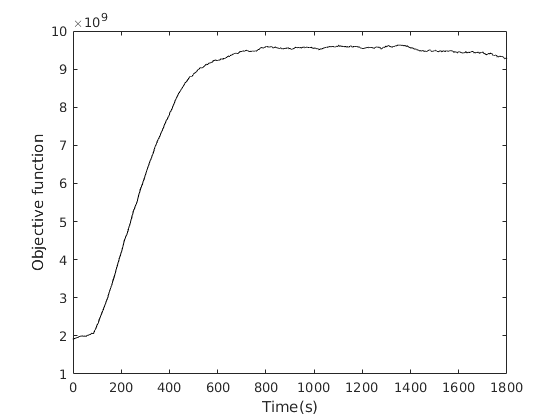
\includegraphics[width=4in]{images/Sobj.eps}
\end{center}
\caption{Objective Function ($\mathbf{E}\left(\mu_{3}^{s}(t) - \mu_{3}^{n}(t)\right)$)} \label{Sobj}
\end{figure}
\begin{figure}[h!] 

\begin{center}
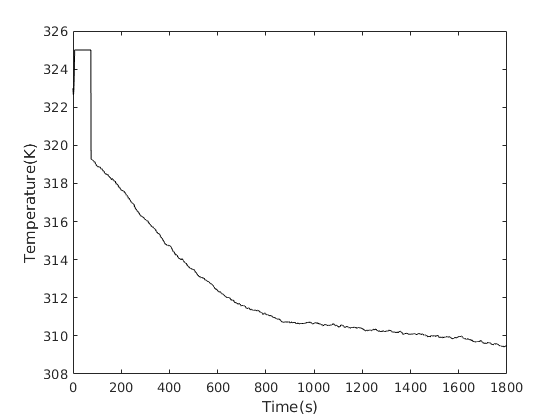
\includegraphics[width=4in]{images/Stemp.eps}
\end{center}
\caption{The optimum cooling profile for the system} \label{Stemp}
\end{figure}

\begin{figure}[h!] 

\begin{center}
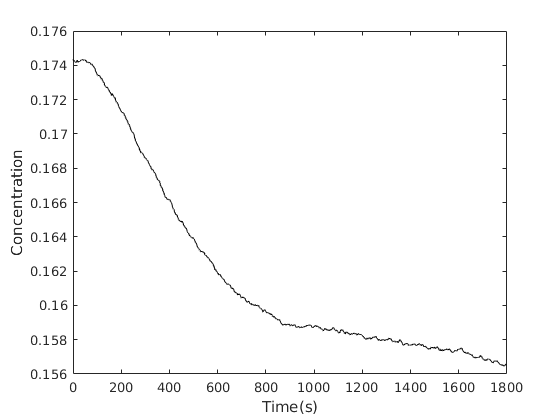
\includegraphics[width=4in]{images/Sconc.eps}
\end{center}
\caption{Concentration Profile}
\end{figure}


\subsection{Stochastic Optimal Control using Polynomial Chaos Expansions}

Polynomial Chaos (PC) expansions (\cite{wiener}) have risen as efficient means of representing stochastic processes with the intention of quantifying uncertainty in differential equations. PC expansions are based on a probabilistic framework and represent stochastic quantities as spectral expansions of orthogonal polynomials. In the following work, we propose the use of PC expansions to propogate uncertainity into the crystallization model and then we compare it's performance with the other methods in this domain. 
%\cite{mesbah,fagiano,huschto,kim2013}

\subsubsection{Mathemetical Background}
The PC expansion can be considered as a mathematical model that is able to solve stochastic problems: the response of a system under stochastic effects which can be represented via a properly constructed basis functions. A stochastic process $Y(x,t,\xi)$ with finite second-order moments and normalized random variables collected in the vector $\xi$ can be represented as follows : 
\begin{equation}
Y(x,t,\xi) = \mathcal{L}(x,t,\xi)
\end{equation}
where $t \in [0, T]$ represents the time, x is the state vector, and $\mathcal{L}$ is an operator (linear or nonlinear).
Now, $Y$ can be expressed as an infinite series of orthogonal basis functions(\cite{ghanem}, \cite{ghanem1997}), $\Phi_{i}$ with suitable deterministic coefficients $a_{i}$ as :
\begin{equation} \label{exact}
Y(t,\xi) =  \sum_{i=0}^{\infty} a_{i}(t)\Phi_{i}(\xi)
\end{equation}
where the representation in (\ref{exact}) is exact. However, for practical applications, Equation (\ref{exact}) is
truncated to a limited number of basis functions M + 1 and is represented as :
\begin{equation} \label{approx}
Y(t,\xi) \approx \sum_{i=0}^{M} a_{i}(t)\Phi_{i}(\xi)
\end{equation}
The total number of terms depends on the number of dimensions, $N$ of the random multivariate parameter $\xi$ and the highest order $P$ of the polynomials $\Phi_{i}$ which is set according to the required accuracy. The number of terms now become $ M + 1 = \frac{(N+P)!}{N!P!} $. The basis functions $\Phi_{i}$ used for generating polynomial expansions  are chosen from the Askey scheme (\cite{xiuwiener}) which maps the polynomial functions to the type of stochastic distribution of the random variables($\xi$) that are considered in the model. In our case the parameters follow a Gaussian distribution (\cite{yenkie}), which uses Hermite Polynomials to describe the probability distribution in the least number of terms.
\par
Thus, given a process model with uncertain output, $y = f(x,\lambda)$, where $x$ is the uncertain input and $\lambda$ is the uncertain parameter, the aim is to quantify uncertainty in $y(\xi)$ from $x(\xi)$ and $\lambda(\theta)$ using the process model. The crystallization model given by Equations \Crefrange{obj}{adjoints} corresponds to these notations as follows. $\lambda$ is the set of uncertain kinetic parameters given in Table \ref{Table2} whereas $\xi$ is a random variable of the gaussian distribution.  

Then the first step is to construct PCE’s of $x(\theta)$, and $\lambda(\theta)$, by determining their PCE coefficients $x_{i}$ and $\lambda_{i}$.
\begin{align}
x(\theta) &= \sum_{i=1}^{P_{PCE}} x_{i}\phi(\theta)
\lambda(\theta) &= \sum_{i=1}^{P_{PCE}} \lambda_{i}\phi(\theta)
\end{align}
\begin{align}
&x_{i} = \frac{\int x\phi_{i}(\theta)g(\theta) d\theta}{\left\langle \phi^{2}_{i}\right\rangle } \quad
&\lambda_{i} = \frac{\int \lambda\phi_{i}(\theta)g(\theta) d\theta}{\left\langle \phi^{2}_{i}\right\rangle }
\end{align}
where $g(\theta)$ is probability distribution function (pdf) of $\theta$. 
The next step is to develop PCE for $y(\theta)$ from  $x(\theta)$, and $\lambda(\theta)$, which can be done by evaluating the
inner product of $y(\theta)$ with each basis functions $\phi_{i}$ to determine the ith- PCE coefficient.
\begin{equation}
y_{i} = \frac{\left\langle f(x,\lambda)\phi_{i} \right\rangle }{\left\langle \phi^{2}_{i} \right\rangle }
\end{equation}
Evaluating the inner product $\left\langle y\phi_{i} \right\rangle $, requires computation of multi-dimensional integrals which can be performed by one of two approaches referred to as \textbf{non-intrusive} and \textbf{intrusive}.
Next, The orthogonality property of the basis functions($\phi_{i}$) is used for the calculation of the coefficients when propagating uncertainty from the input random variables $\xi$, to the output variables ($Y$).
\par
\subsubsection{Usage of PCE in Batch Crystallization}

Extending the concepts from the previous section, the state varibles($y_{i}$)(\Crefrange{eq1}{eq9}) act as the uncertain outputs which is caused by uncertainities present in process parameters $\lambda$ ($k_{g}, E_{g}, g, k_{b}, E_{b}, b$), used to calculate the Growth rate ($G(t) = k_{g}\exp{\left(-E_{g}/RT \right)}\left(\frac{C - C_{s}(T)}{C_{s}(T)}\right)^{g}$) and the Nucleation rate ($B(t) = k_{b}\exp{\left(-E_{b}/RT \right)}\left(\frac{C - C_{s}(T)}{C_{s}(T)}\right)^{b}\mu_{3}$). Temperatue($T(t)$) acts as the input variable $x$ in the above system. The PC expansion coefficients can be determined using the probabilistic collocation methods. Using these methods, N samples are drawn from the known distributions of uncertainties and, subsequently, are used to solve the nonlinear process model \Crefrange{obj}{adjoints}. The PC expansion coefficients can then be obtained in a least squares sense by minimizing the residuals between the PC expansion and the nonlinear model predictions. The complete algorithm is mentioned below.

\textbf{Algorithm}:
\begin{enumerate}

\item Following the general representation, $y_{i}$ can be written as :
\begin{align*}
y_{i} = f(x(\theta),\lambda_{i}(\theta))
\end{align*}
where x is the input temperature(T), $\lambda_{i}$'s are process parameters and $\theta$ is the random variable.
%% Can add a example expression here
\item The process model consists of 6 uncertainities which computationally prohibits the evaluation. Thus, an approximation of $n_{0} = 2$ is taken by employing a joint distribution of the parameters.
\item Samples are generated for the model at $N$ points. The sampling technique used is the Gaussian Quadratures along with Hermite Polynomials to represent state variables $(y_{i})$ into Eq(5.17).

\item For each of the above sample $y^{j}_{i} = f(T^{j}(\theta),\lambda(\theta) $ ,  the optimization problem is solved using the Steepest Ascent Hamiltonian method discussed in Section(4.1.1).

\item The optimum value of the input temperature $T^{j}(\theta)$ at these samples is used to construct the PCE's for $T(\theta)$ and $\lambda(\theta)$ as given by Equations(5.18).

\item $y^{j}_{i}$'s for each sample are used to evaluate :
\begin{equation}
y_{i} = \frac{1}{\left\langle \phi^{2}_{i}\right\rangle }\frac{1}{N} \sum_{j=1}^{N} y^{j}\phi_{i}(\theta)
\end{equation}
Here, $\phi_{i}$ are the coefficients of the orthogonal polynomials being used for PCE estimation.  

\item As the above Equation averages over N samples, the resultant $y_{i}$ maximises the objective function, given by $ \mathbf{E} \left\lbrace  y_{5}-y_{9} \right\rbrace $). 

\end{enumerate} 

\subsubsection{Results}

All the source scripts for using PCE with the crystallization model were written Python, using the open source library \textbf{chaospy}\cite{chaospy}. It is a toolbox for performing uncertainity quantification through polynomial chaos expansions and efficient sampling strategies. The base model for performing simulations was derived from Section \ref{secdet}. The range of values exhibited by the uncertain parameters have been mentioned in the Table \ref{Table3}. The results obtained can be observed from \cref{PCEConc}



%\begin{figure}[h!] 

%\begin{center}
%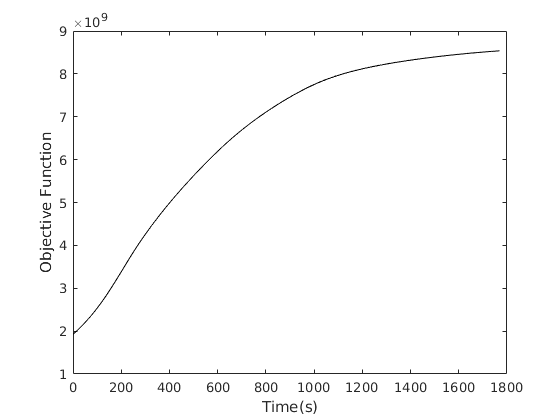
\includegraphics[width=4in]{images/PCEobj.eps}
%\end{center}
%\caption{Objective Function ($\mathbf{E}\left[\mu_{3}^{s}(t) - \mu_{3}^{n}(t)\right]$)}
%\end{figure}
%\begin{figure}[h!] 

%\begin{center}
%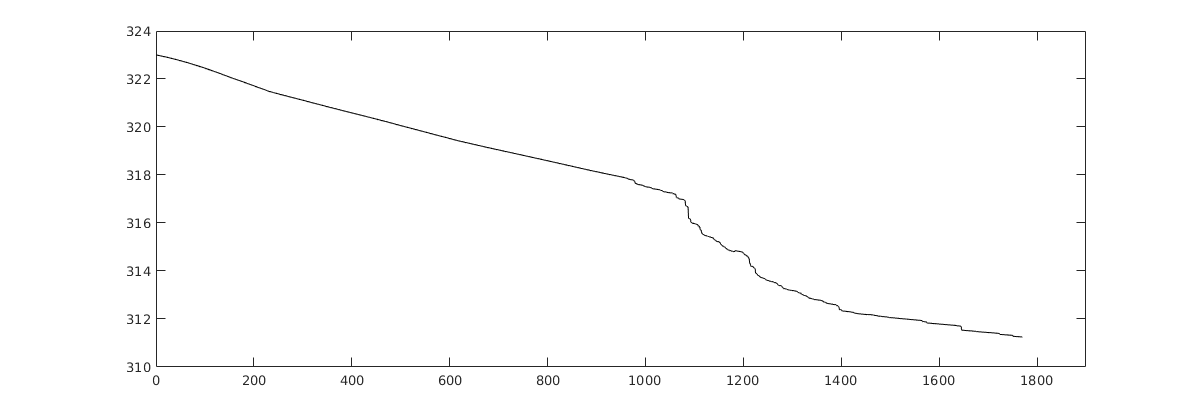
\includegraphics[width=4in]{images/PCETemp.eps}
%\end{center}
%\caption{The cooling profile for the controlled variable T(t) obtained at the final iteration}
%\end{figure}

\begin{figure}[h!] 

\begin{center}
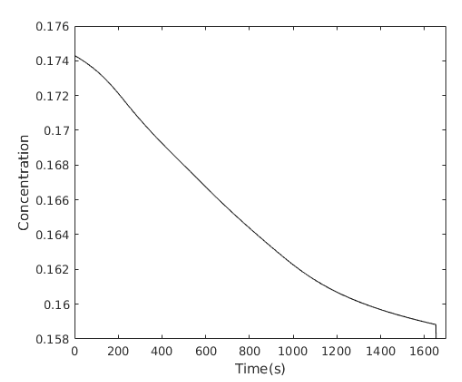
\includegraphics[width=4in]{images/PCEConc.eps} \label{PCEConc}
\end{center}
\caption{The Concentration profile}
\end{figure}

\section{Case Study}

In the following case study we aim to build a predictive model for batch crystallization of L-Asparagine Monohyrdate(LAM) by using the concepts developed in the previous section and at the same time validate the performance of Polynomial Chaos Expansions (PCEs) on an unseeded batch crystallization scenario.   

\subsection{Mathematical Background}


The kinetics of crystal formation are modeled using the population balance equations(PBE) in \ref{populationbalance}, where the nucleation rate expression for LAM crystals is given by \cite{lindenberg} :
\begin{equation}
B = k_{j_{1}}S\exp\left( -k_{j_{2}}\frac{\ln^{3}{C_{c}/C^{*}}}{\ln^{2}S}\right) 
\end{equation}
in which $C_{c}$ represents the  molar density of LAM crystals. Here, $k_{j_{1}}$ and $k_{j_{2}}$ are
empirical parameters. The growth rate (\cite{nagy} and \cite{nagy2}) is now given by the power-law expression in \ref{newgrowth}. 
\begin{equation}
G = k_{g}(S-1)^{g} \label{newgrowth}
\end{equation}
The supersaturation ratio, S, is defined as :
\begin{equation}
S = C/C^{*}
\end{equation}
where $C^{*}$ represents the saturation concentration of LAM crystals. The solubility of these crystals can be expressed as:
\begin{equation}
C^{*} = 5 \times 10^{-5}T^{2} - 0.001T + 0.0236
\end{equation}
The experimental values for the set of kinetic parameters $[k_{g}, g, k_{j_{1}}, k_{j_{2}}]$ (\cite{bhoi}) have been mentioned in the Table \ref{Table4} .

\begin{center}
\begin{table}[!h]
\centering 
\caption{Kinetic Parameters} \label{Table4}
\begin{tabular}{|c|c|c|}
\hline
Parameters & Experimental Values & Range of Values\\
\hline
\multicolumn{3}{|c|}{Growth Kinetics} \\
\hline
$\ln(k_{g})$ & $3.41\pm 0.28$ & $\mu m min^{-1} $\\
$g$ & $1.48\pm 0.04$ & $ - $\\
\hline
\multicolumn{3}{|c|}{Nucleation Kinetics} \\
\hline
$\ln(k_{j_{1}})$ & $24.74\pm0.73$ & $No. per m^{3}min$\\ 
$k_{j_{2}}$ & $2.7\times10^{-2}\pm 3.2\times10^{-3}$ & $-$\\
\hline
\end{tabular}

\label{values}
\end{table}
\end{center}

Method of Moments has been used to reduce the PBE to ODE's as stated in Section \ref{modeleq}. The mass balance for LAM crystals also remains the same from there, with the difference being the absence of seeded crystals.\\

The ODEs for the model are given by :
\begin{align}
\frac{du_{0}}{dt} &= B \\
\frac{du_{j}}{dt} &= jG\mu_{j-1}
\end{align}
for  $j = 1,2,3,4 $ \\
The determination of the optimal temperature profile for maximizing the weight mean size is a highly studied objective for a crystallization process.Thus, 
\paragraph{Objective Function} becomes :
\begin{align}
\max_{T(t)}	\phi = \mu_{4}/\mu_{3} \quad at \quad t_{f} 
\end{align}
\paragraph{Constraints}
\begin{align}
T_{min} &\leqslant T(t) \leqslant T_{max} \\
\frac{dT}{dt} &\leqslant 0
\end{align}
The state variables can be represented as :
\begin{equation*}
y_{i} = \left[\quad C \quad \mu_{0} \quad \mu_{1} \quad \mu_{2} \quad \mu_{3}\quad \mu_{4} \quad\right]  
\end{equation*}
Here we do not divide the moments in seeded and nucleated ones.\\
The Hamiltonian method described in the previous sections was employed to solve the optimaization problem along with the uncertainity quantification being done using Polynomial Chaos Expansions. The new state equations, constraints and kinetics as described above are used to define the problem.\\

\subsection{Solution Technique : Hamiltonian Steepest Ascent with PCE}

Equations(6.5-6.6) take place as the new state equations and the uncertain parameters are mentioned in Table 6.1. The constraint(Eq 6.9)) depicts a cooling profile for the crystallizer. The obejective function here (Eq 6.7) differs from the one used in Section(\ref{deterministic}) so as to calculate the final maximum mean size of the crystals.\\ 
Key Differences :
\begin{itemize}
\item The batch time for the model was taken to be 240 min($t_{f}$).
\item An initial concentration value of 0.073 $g/L$ was taken to obtain the cooling profile. All the moments were intialised to 0.
\item The ODEs were integrated using Python \textbf{scipy's} \textbf{odeint} integrator.
\end{itemize}

\paragraph{Algorithm}
\begin{enumerate}
\item The process model consists of 4 uncertainities which computationally prohibits the evaluation. Thus, the experiment has been done on $k_{g}$ and $g$, employing a joint distribution of the parameters.
\item Samples are generated using the distribution using Gaussian Quadrature Scheme.
\item The function is evaluated at each of these samples to evalute the integrals numerically to determine the PCE coefficients.
\item At each sample, optimization of the model is performed using the Determinstic Approach explained in Section(\ref{deterministic}).
\item The convergence criteria and the constraints remain same as the above referenced method.
\end{enumerate}

\subsection{Results}
The value for the concentration profile for the time horizon was obtained as :
\begin{figure}[h!] 
\begin{center}
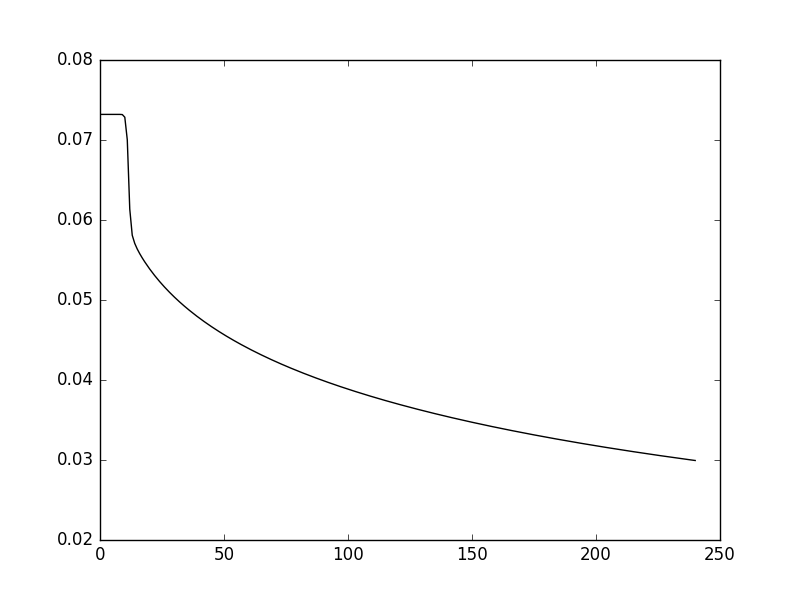
\includegraphics[width=4in]{AppConc.png}
\end{center}
\caption{Concentration Profile}
\end{figure}

The value for the temperature profile was obtained as :
\begin{figure}[h!] 
\begin{center}
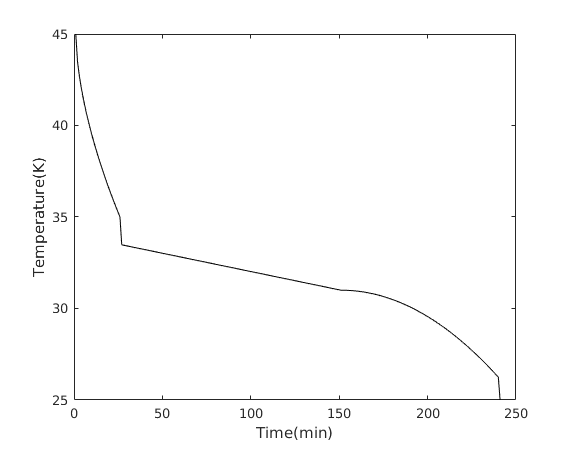
\includegraphics[width=4in]{AppTemp.png}
\end{center}
\caption{Temperature Profile}
\end{figure}

\subsection{Conclusion}

\begin{itemize}
\item The final value of the objective function($\mu_{4}/\mu_{3}$), ie. the mean crystal size was obtained at : $300 \mu m$
\item The model performs at par with other cooling policies such as cubic cooling policy($251 \mu m$)\cite{bhoi}. This proves the efficacy of P.C.E in the field of batch crystallization.
\end{itemize}


\section{Conclusion}




%% The Appendices part is started with the command \appendix;
%% appendix sections are then done as normal sections
%% \appendix

%% \section{}
%% \label{}

%% References
%%
%% Following citation commands can be used in the body text:
%% Usage of \cite is as follows:
%%   \cite{key}         ==>>  [#]
%%   \cite[chap. 2]{key} ==>> [#, chap. 2]
%%

%% References with BibTeX database:

\clearpage
\section{References}

\bibliography{mybibfile}
% Authors are advised to use a BibTeX database file for their reference list.
%% The provided style file elsarticle-num.bst formats references in the required Procedia style

%% For references without a BibTeX database:
%
%\newpage
%\section{References}
%\begin{thebibliography}{1}

%\bibitem must have the following form:
% \bibitem{key}...
	
 %\bibitem{}

%\end{thebibliography}

\end{document}

%%
%% End of file `ecrc-template.tex'. 